\documentclass[fleqn,10pt]{wlscirep}
\usepackage[utf8]{inputenc}
\usepackage[T1]{fontenc}

\usepackage{apjfonts}

\usepackage{lipsum}  

%\received{\today}
%\revised{\today}
%\accepted{\today}
%% Command to document which AAS Journal the manuscript was submitted to.
%% Adds "Submitted to " the argument.
%\submitjournal{AJ}

%\topmargin 0.6in

\usepackage{xspace}
\usepackage{multirow}
\usepackage{natbib}
%\usepackage[dvipsnames]{xcolor}

%\usepackage{deluxetable}
%\usepackage{color}
%\definecolor{citeRGB}{rgb}{0,0.1,0.7}
%\usepackage[hyperfootnotes=true,naturalnames=true,letterpaper,pdfstartview=FitH,pdfpagemode=UseNone,colorlinks=true,citecolor=citeRGB]{hyperref}

\gdef\HST{\textit{HST}}
\gdef\Spitzer{\textit{Spitzer}}
\gdef\fluxcgs{\mathrm{erg~s^{-1}~cm^{-2}}}
\gdef\micront{$\mu$m}
\gdef\micronm{\mu\mathrm{m}}
\gdef\aXe{\texttt{aXe}}
\gdef\fluxradius{\textsc{flux\_radius}}
\gdef\epers{\textit{e}$^{-}$ s$^{-1}$}

%\gdef\logOH{12 + \log \left(\mathrm{O/H}\right)}
\gdef\SFRuvir{SFR_\mathrm{UV+IR}}
\gdef\peryr{\mathrm{yr}^{-1}}
\gdef\kms{km\,s$^{-1}$}
\gdef\mum{$\mu\mathrm{m}$}
\gdef\24mum{$24\,\mu\mathrm{m}$}
\gdef\arcsec{^{\prime\prime}}
\gdef\UDFj{UDFj-39546284}
\gdef\compareID{UDF-40106456}
%\gdef\Lya{\mathrm{Ly}\alpha}
%\gdef\Halpha{\mathrm{H}\alpha}
%\gdef\Hbeta{\mathrm{H}\beta}

\newcommand\xxx{{\textcolor{red}{\bf xxx}}}
\newcommand\xref[1]{{\textcolor{red}{\bf (REF #1)}}}
\newcommand\XXX[1]{{\textcolor{red}{xxx #1}}}

%%   DEFINE YOUR OWN CUSTOM COMMENT COMMAND HERE:
\newcommand\SR[1]{{\authorcomment2{\textcolor{red}{SR: #1}}}}
\newcommand\JP[1]{{\authorcomment2{\textcolor{blue}{JP: #1}}}}


\gdef\HAWKI{\mbox{HAWK-I}}

\gdef\sncode{\mbox{ABC}}

\shortauthors{XXX et al.}
\shorttitle{CHArGE}
% \setwatermarkfontsize{50pt} 
%\citestyle{aa}



%% PLACEHOLDER FOR THE SN Nickname or TNS designation
\def\SNABC{SN Requiem\xspace}

\title{Three magnified views of a supernova explosion 10 billion years ago, and a fourth that will reveal the nature of cosmological dark energy}

\author[1,*]{Gabriel Brammer}
\author[2]{Steven Rodney}
\author[2]{Justin Pierel}
\author[2]{Kyle O'Connor}
\author[3]{Johan Richard}
\author[1]{Sune Toft}
\author[4]{Mohammad Akhshik}
\author[5]{Katherine Whitaker}
\affil[1]{Cosmic Dawn Center, Niels Bohr Institute, K{\o}benhavns Universitet}
\affil[2]{University of South Carolina}
\affil[3]{Universit\'e Claude Bernard Lyon}
\affil[4]{University of Connecticut}
\affil[5]{University of Massachusetts, Amherst}

\affil[*]{gabriel.brammer@nbi.ku.dk}

%\affil[+]{these authors contributed equally to this work}

%\keywords{Keyword1, Keyword2, Keyword3}

\begin{abstract}
% https://www.nature.com/documents/nature-summary-paragraph.pdf
%One or two sentences providing a basic introduction to the field, comprehensible to a scientist in any discipline
The expansion history of the Universe is one of the most fundamental observations leading to the hot big bang model for the origin of the Universe. 
%Two to three sentences of more detailed background, comprehensible to scientists in related disciplines.
The observed brightness of distant Type Ia supernova (SN) explosions has played a key role in mapping the expansion history, and led to the discovery of dark energy that now appears to be driving an accelerating cosmic expansion rate.
Determining the nature of dark energy and how it may evolve over time is a primary goal for current and planned large-scale cosmology experiments.
%One sentence clearly stating the general problem being addressed by this particular study
One promising method for determining the dark energy equation of state and its evolution  is through time delays of gravitational lens systems, which for a given lens potential provide a measurement of the ratio of the angular diameter distances to the foreground lens and background source.
%One sentence summarising the main result (with the words “here we show” or their equivalent).
Here we report the discovery of a strongly-lensed Type Ia SN explosion that will provide a time delay precision of $<1\%$.  The SN is in an evolved galaxy at $z=1.95$ gravitationally lensed by a massive foreground galaxy cluster.
%Two or three sentences explaining what the main result reveals in direct comparison to what was thought to be the case previously, or how the main result adds to previous knowledge.
With three lensed images of the supernova detected in existing observations from the \textit{Hubble Space Telescope} with time delays of order 50 days, this is the most distant multiply-imaged supernova yet discovered.  A fourth image in the component closest to the cluster core is predicted to appear in the year 2035$\pm$2.  Observing the lightcurve of that future image will provide a time delay precision of $\approx 7$ days over an unprecedented baseline of nearly 20 years.  This single source will therefore provide a similar precision and complementary cosmological constraints to an ensemble of dozens of time delay measurements expected at somewhat lower redshifts and shorter timescales from the planned ground-based LSST and WFIRST space telescope missions.  If we suppose that cosmological parameters such as the local expansion rate ($H_0$) and dominant energy densities $\Omega_m$ and $\Omega_\Lambda$ will be well established in 2035, the combined time delay measurements will constrain the dark energy equation of state ($w_0$) to better than 10\%.
%One or two sentences to put the results into a more general context. 
% Considering this observation in the context of
% Two or three sentences to provide a broader perspective, readily comprehensible to a scientist in any discipline, may be included in the first paragraph if the editor considers that the accessibility of the paper is significantly enhanced by their inclusion.

\end{abstract}
\begin{document}

\flushbottom
\maketitle

%
%  Click the title above to edit the author information and abstract
%

% \thispagestyle{empty}

% \section*{Introduction}

% \section*{Results}

%Up to three levels of \textbf{subheading} are permitted. Subheadings should not be numbered.

%\subsection*{Subsection}

% Example text under a subsection. Bulleted lists may be used where appropriate, e.g.

% \begin{itemize}
% \item First item
% \item Second item
% \end{itemize}

% \subsubsection*{Third-level section}
 
% Topical subheadings are allowed.

% \section*{Discussion}

% The Discussion should be succinct and must not contain subheadings.

% \section*{Methods}

% Topical subheadings are allowed. Authors must ensure that their Methods section includes adequate experimental and characterization data necessary for others in the field to reproduce their work.

% \bibliography{sample}

% \noindent LaTeX formats citations and references automatically using the bibliography records in your .bib file, which you can edit via the project menu. Use the cite command for an inline citation, e.g.  \cite{Hao:gidmaps:2014}.

% For data citations of datasets uploaded to e.g. \emph{figshare}, please use the \verb|howpublished| option in the bib entry to specify the platform and the link, as in the \verb|Hao:gidmaps:2014| example in the sample bibliography file.

% \section*{Acknowledgements (not compulsory)}

% Acknowledgements should be brief, and should not include thanks to anonymous referees and editors, or effusive comments. Grant or contribution numbers may be acknowledged.

% \section*{Author contributions statement}

% Must include all authors, identified by initials, for example: A.A. conceived the experiment(s),  A.A. and B.A. conducted the experiment(s), C.A. and D.A. analysed the results.  All authors reviewed the manuscript. 

% \section*{Additional information}

% To include, in this order: \textbf{Accession codes} (where applicable); \textbf{Competing interests} (mandatory statement). 

% The corresponding author is responsible for submitting a \href{http://www.nature.com/srep/policies/index.html#competing}{competing interests statement} on behalf of all authors of the paper. This statement must be included in the submitted article file.

\begin{figure*}
    \centering
    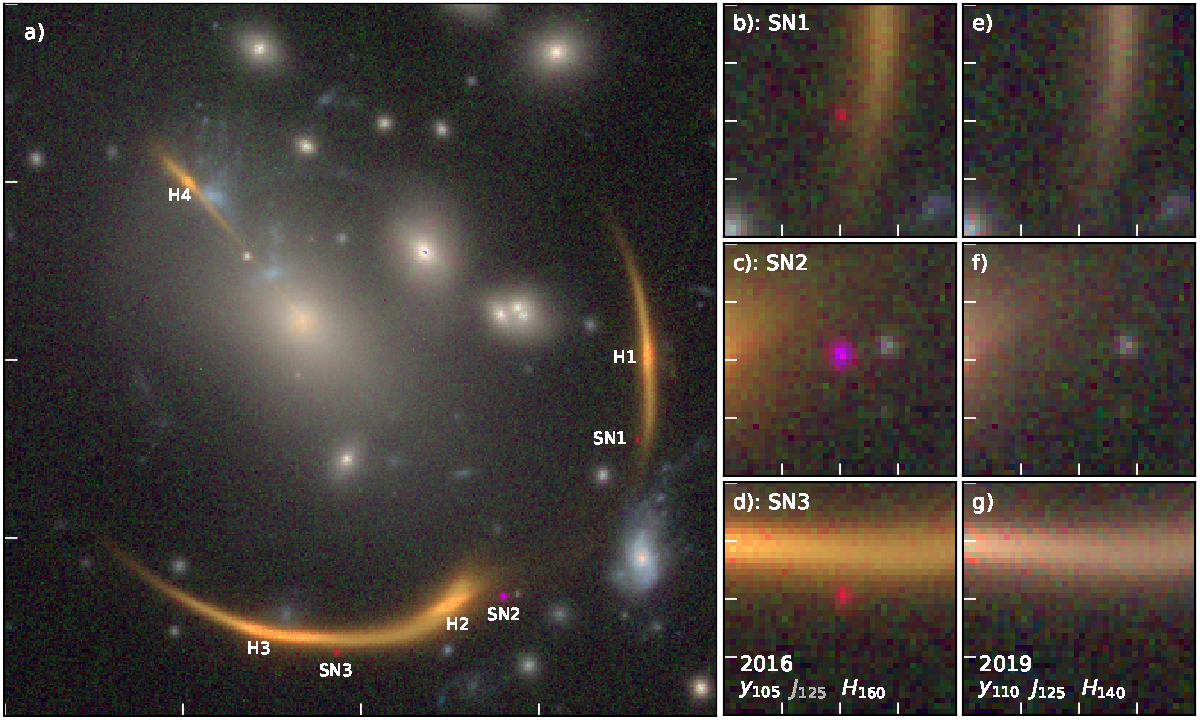
\includegraphics[width=0.9\textwidth]{../Figures/fig1_layout.pdf}
    \caption{Overview of the field around the center of the MACSJ0138 cluster field and the locations of the lensed host (H1--4) and \SNABC (SN1--3) images. 
    %The wide-field view in $a)$ is 40\arcsec\ on a side with ticks indicating 10\arcsec\ intervals.  Panels b--g) show 4\arcsec\ cutouts around the lensed SN images with 1\arcsec\ ticks.  
    Three-color images are generated from the \textit{Hubble} WFC3/IR filters as indicated; panels $b$--$d$ show the imaging from July 2016 where the SN was visible and $e$--$g$ show the later imaging from July 2019 where the the SN has faded away.  It is immediately clear that the SN2 image is substantially bluer than the other two, which helps constrain the transient classification as a likely Ia supernova explosion.  \textbf{The lens model that predicts time delays of the first three images consistent with the evolution of the Ia lightcurve predicts that the SN image in H4 will appear in 2035.} }
    \label{fig:layout}
\end{figure*}

\begin{figure*}
    \centering
    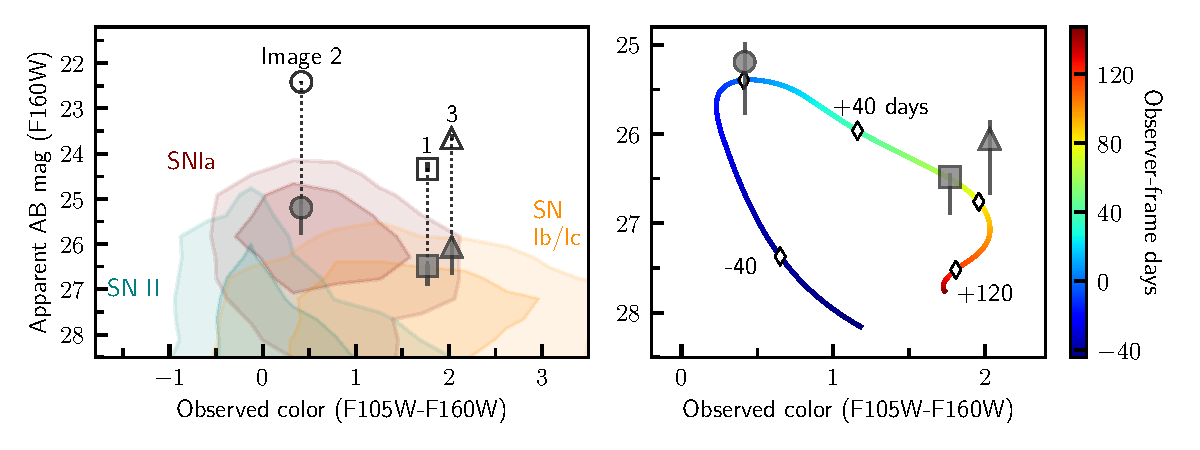
\includegraphics[width=\textwidth]{Paper/Figures/classification_contours_timeline.pdf}
    \caption{Classification information for \SNABC based on its position in color-magnitude space. (left) Contours show the population distributions for normal SNe of Type Ia (red), Type Ib/Ic (gold), and Type II (green).  These population contours are drawn to enclose 68\% (interior solid lines) and 95\% (exterior shaded regions) of each SN population.  Each SN sub-class was simulated at $z=1.95$, and samples from their expected light curves were drawn uniformly in time. Open markers show the observed photometry of the SN. Dotted vertical lines mark the magnification correction based on the lens modeling, terminating in closed markers with error bars that show the magnitude uncertainty, which is dominated by the lens modeling uncertainty.  (right) The evolution of a Type Ia SN at $z=1.95$ in observed color-mag space is shown by a colored line, with the color indicating SN age in observer-frame days relative to peak brightness.  White diamonds correspond to the labels on the colorbar at right, showing the time relative to maximum brightness in the observer frame. An interactive 3-D version of this figure is available online \href{https://plot.ly/~jpierel/6/#/}{here}.
    }
    \label{fig:colormag}
\end{figure*}


% \begin{figure}
%     \centering
%     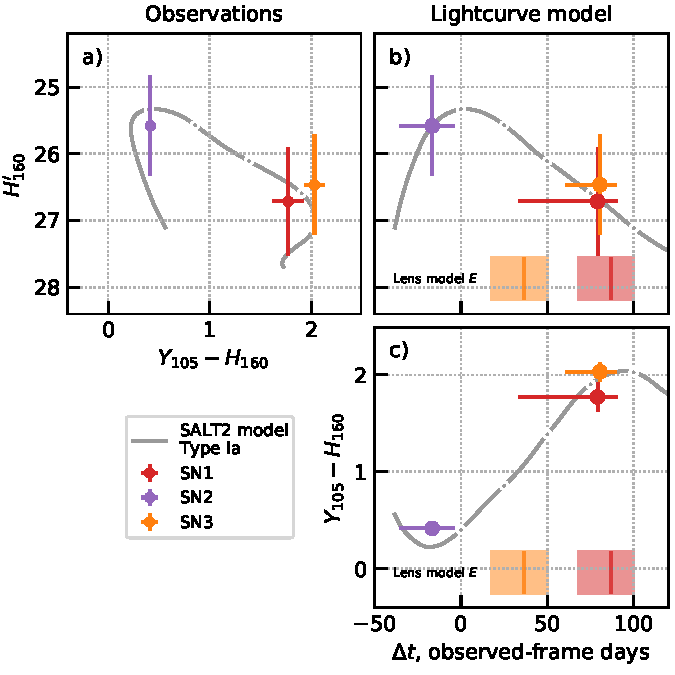
\includegraphics[width=0.5\textwidth]{../Figures/combined_lightcurve.pdf}
%     \caption{Color and magnitude evolution from the multiple images of the SN. Panel $a)$ shows the direct measurements for the three SN images, where the $H_{160}$-band magnitude has been corrected for the (achromatic) gravitational lensing magnification derived from the lens model.  The evolution in both color and magnitude is fully consistent with a Type Ia template (gray curve) where the SN2 image is observed just before peak brightness and the other two images show the SN approximately 30 rest-frame days after the peak. These time delays inferred from the lightcurve are consistent with the estimates from the lens model, shown in the filled regions at lower right.}
%     \label{fig:my_label}
% \end{figure}

\begin{figure}
    \centering
    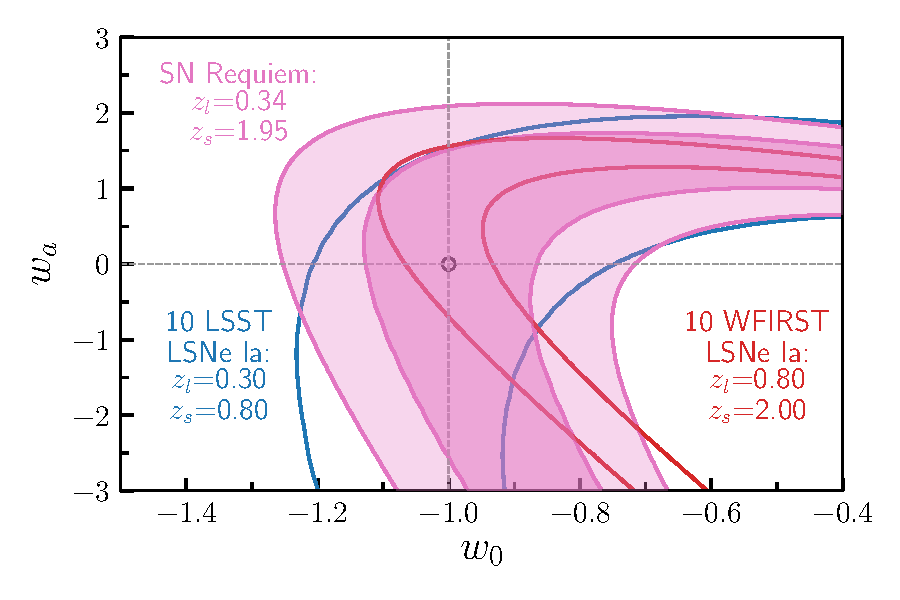
\includegraphics[width=0.7\textwidth]{../Figures/snrequiem_w0wa_compared_to_lsst_wfirst.pdf}
    \caption{The unusual sensitivity of SN Requiem to dark energy equation of state parameters ($w_0, w_a$). Contours show the 1$\sigma$ confidence region for a typical sample of lensed SNIa time delays from LSST (blue) and WFIRST (red) compared to SN Requiem (magenta). Dashed lines and the white marker show the input values of $w_0=-1$, $w_a=0$ that were used for this simulation. In order to isolate the $w_0, w_a$ dependence, all contours are constructed assuming perfect knowledge of $H_0$, $\Omega_{m,0}$ and $\Omega_{\rm de,0}$.  SN Requiem could be highly complementary to the LSST+WFIRST lensed SN sample, due to its unusual combination of a relatively low-redshift lens ($z=0.338$) and high-redshift source ($z=1.95$). This single SN could deliver constraints on dark energy equation of state parameters comparable to several dozen SNe with shorter and less precise  time delays.}
    \label{fig:my_label}
\end{figure}

% \begin{figure}[ht]
% \centering
% \includegraphics[width=\linewidth]{stream}
% \caption{Legend (350 words max). Example legend text.}
% \label{fig:stream}
% \end{figure}

% \begin{table}[ht]
% \centering
% \begin{tabular}{|l|l|l|}
% \hline
% Condition & n & p \\
% \hline
% A & 5 & 0.1 \\
% \hline
% B & 10 & 0.01 \\
% \hline
% \end{tabular}
% \caption{\label{tab:example}Legend (350 words max). Example legend text.}
% \end{table}

% Figures and tables can be referenced in LaTeX using the ref command, e.g. Figure \ref{fig:stream} and Table \ref{tab:example}.

\end{document}